\documentclass[12pt, a4paper]{article}
\usepackage[utf8]{inputenc}
\usepackage[english]{babel}
\usepackage{amsmath}
\usepackage{amsfonts}
\usepackage{amssymb}
\usepackage{fvextra}
\usepackage{csquotes}
\usepackage{mathtools}
\usepackage{graphicx}
\usepackage{geometry}
\usepackage{setspace}
\usepackage{longtable}
\usepackage{float}
\usepackage{comment}
\usepackage{minted}
\usepackage{fancyhdr}
\usepackage{siunitx}
\usepackage[T1]{fontenc}
\usepackage{|modern}
\usemintedstyle{bw}
\usepackage[colorlinks=true, allcolors=blue]{hyperref}

\usepackage[style=authoryear]{biblatex}
\addbibresource{Bibliography.bib}

\geometry{top = 2.5cm, bottom = 2.5cm, left= 3cm, right= 3cm}

\fancypagestyle{mystyle}
{
    \rhead{Experiment 8}
    \lfoot{Lee Farrugia}
    \cfoot{}
    \rfoot{Page \thepage}
    \renewcommand{\headrulewidth}{0pt}
    \renewcommand{\footrulewidth}{0.5pt}
}

\fancypagestyle{titlepagestyle}
{
    \fancyhf{}
    \lfoot{Lee Farrugia}
    \cfoot{}
    \rfoot{Page \thepage}
    \renewcommand{\headrulewidth}{0pt}
    \renewcommand{\footrulewidth}{0.5pt}
}

\title{Verification of Cauchy's equation}
\author{Lee Farrugia \\ Experiment 8 \\ Group 1A}

\date{6$^{\text{th}}$ May 2022}

\begin{document}

\maketitle
\thispagestyle{titlepagestyle}
\pagestyle{mystyle}

\section*{Aim}
The aim of this experiment was to determine the dependence of the refractive index on the wavelength using Cauchy's equation.

\section*{Diagram}
\begin{figure}[H]
    \centering
    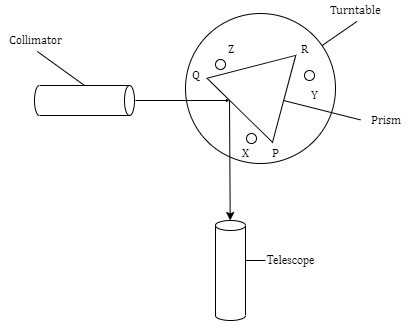
\includegraphics[width = \textwidth]{Experiment 8 Diagram.png}
    \caption{Apparatus set up}
    \label{fig:Set up}
\end{figure}

\section*{List of Apparatus}
Spectrometer, prism, cadmium lamp, power supply, lens and lamp with red covering.

\section*{Language and Packages}
Python 3.10.4, Numpy, Sympy, Math, Matplotlib.pyplot, Pandas.

\section*{Procedure}
\begin{enumerate}
    \item The spectrometer was taken outside in order to be focused on the Chemistry building. A tutor was asked to confirm that the spectrometer was properly focused.
    \item The glass prism was mounted on the spectrometer table and the spectrometer was set up. The cadmium source was placed in the bulb holder and turned on. The apparatus was aligned.
    \item In order to determine the apex angle, $\alpha$, first the frosted side of the prism was placed at six o'clock to the direction of the light coming from the lamp. Then the telescope was aligned with one of the unfrosted faces of the prism and turned until the light from the lamp was located, by means of total internal reflection, the angles of the telescope as seen on the spectrometer were noted below. The same was done on the other unfrosted side and the apex angle was determined.
    \item The minimum angle of deviation was determined next. This was done by first placing the frosted side to ten o'clock to the incoming light from the lamp. When looking through the telescope the crosshair was placed on the red fringe. The prism table and the telescope were turned together in the same direction so as to keep the crosshair in line with the red fringe. At a point the red fringe stopped and turned back on itself, the angles of the telescope were noted and the same was repeated for all the other three colours. This procedure was repeated for all four colour but first setting the frosted side of the prism to two o'clock of the incoming light.
\end{enumerate}

\section*{Precautions}
\begin{itemize}
    \item[-] The room was as dark as possible.
    \item[-] The opening of the lamp was shielded as much as possible.
    \item[-] Time was allowed to pass before viewing the fringes, as to allow the eye to adjust to the darkness.
    \item[-] A lamp was covered with red plastic as to limit the amount of light when reading from the verniers. 
    \item[-] The spectral lamp was turned on from before hand, in order to allow it to reach its maximum temperature.
    \item[-] When taking reading from the verniers, it was made sure that the telescope and the prism table were locked in place. 
    \item[-] The fine adjust was used in order to obtain the best possible reading when placing the crosshair on the centre of the fringe.
    \item[-] The prism was locked into place on the table.
\end{itemize}

\section*{Sources of Error}
\begin{itemize}
    \item[-] Over time with repeated use the lamp may have become dimmer.
    \item[-] The spectrometer although calibrated at a distance, it was not calibrated at infinity.
    \item[-] Even though the room was as dark as possible some light might have had entered. 
    \item[-] The prism used was chipped. 
    \item[-] The verniers might not have been read at eye-level due to the use of the lamp and the lens.
    \item[-] The zero scale error of the verniers.
    \item[-] As the fringe turned back on itself, it was very hard to obtain the exact position that the fringe turns on itself. 
\end{itemize}

\section*{Data and Graphs}
\renewcommand*{\arraystretch}{1.2}
\begin{longtable}{|c|c|c|c|}
\caption{Data of apex angle}
\label{Tab: Table 1}\\
\hline $A/^{\circ}$ & $B/^{\circ}$ & $A'/^{\circ}$ & $B'/^{\circ}$\\
\hline \textpm $\frac{1}{120}$ & \textpm $\frac{1}{120}$ & \textpm $\frac{1}{120}$ & \textpm $\frac{1}{120}$\\ \hline
\endfirsthead

\hline $A/^{\circ}$ & $B/^{\circ}$ & $A'/^{\circ}$ & $B'/^{\circ}$\\
\hline \textpm $\frac{1}{120}$ & \textpm $\frac{1}{120}$ & \textpm $\frac{1}{120}$ & \textpm $\frac{1}{120}$\\ \hline
\endhead

187.67 & 7.72 & 307.45 & 127.47\\\hline
\end{longtable}

\begin{longtable}{|c|c|c|c|c|}
\caption{Data of minimum angle of deviance}
\label{tab: Table 2}\\
\hline $Colour$ & $A/^{\circ}$ & $B/^{\circ}$ & $A'/^{\circ}$ & $B'/^{\circ}$\\
\hline & \textpm $\frac{1}{120}$ & \textpm $\frac{1}{120}$ & \textpm $\frac{1}{120}$ & \textpm $\frac{1}{120}$\\ \hline
\endfirsthead

\hline $Colour$ & $A/^{\circ}$ & $B/^{\circ}$ & $A'/^{\circ}$ & $B'/^{\circ}$\\
\hline & \textpm $\frac{1}{120}$ & \textpm $\frac{1}{120}$ & \textpm $\frac{1}{120}$ & \textpm $\frac{1}{120}$\\ \hline
\endhead

Red & 115.08 & 295.08 & 15.42 & 195.43\\ \hline
Green & 116.25 & 296.25 & 14.37 & 194.38 \\ \hline
Cyan & 116.70 & 296.70 & 14.70 & 194.70 \\ \hline
Blue & 117.50 & 297.50 & 13.93 & 193.33 \\\hline
\end{longtable}

\begin{figure}
    \centering
    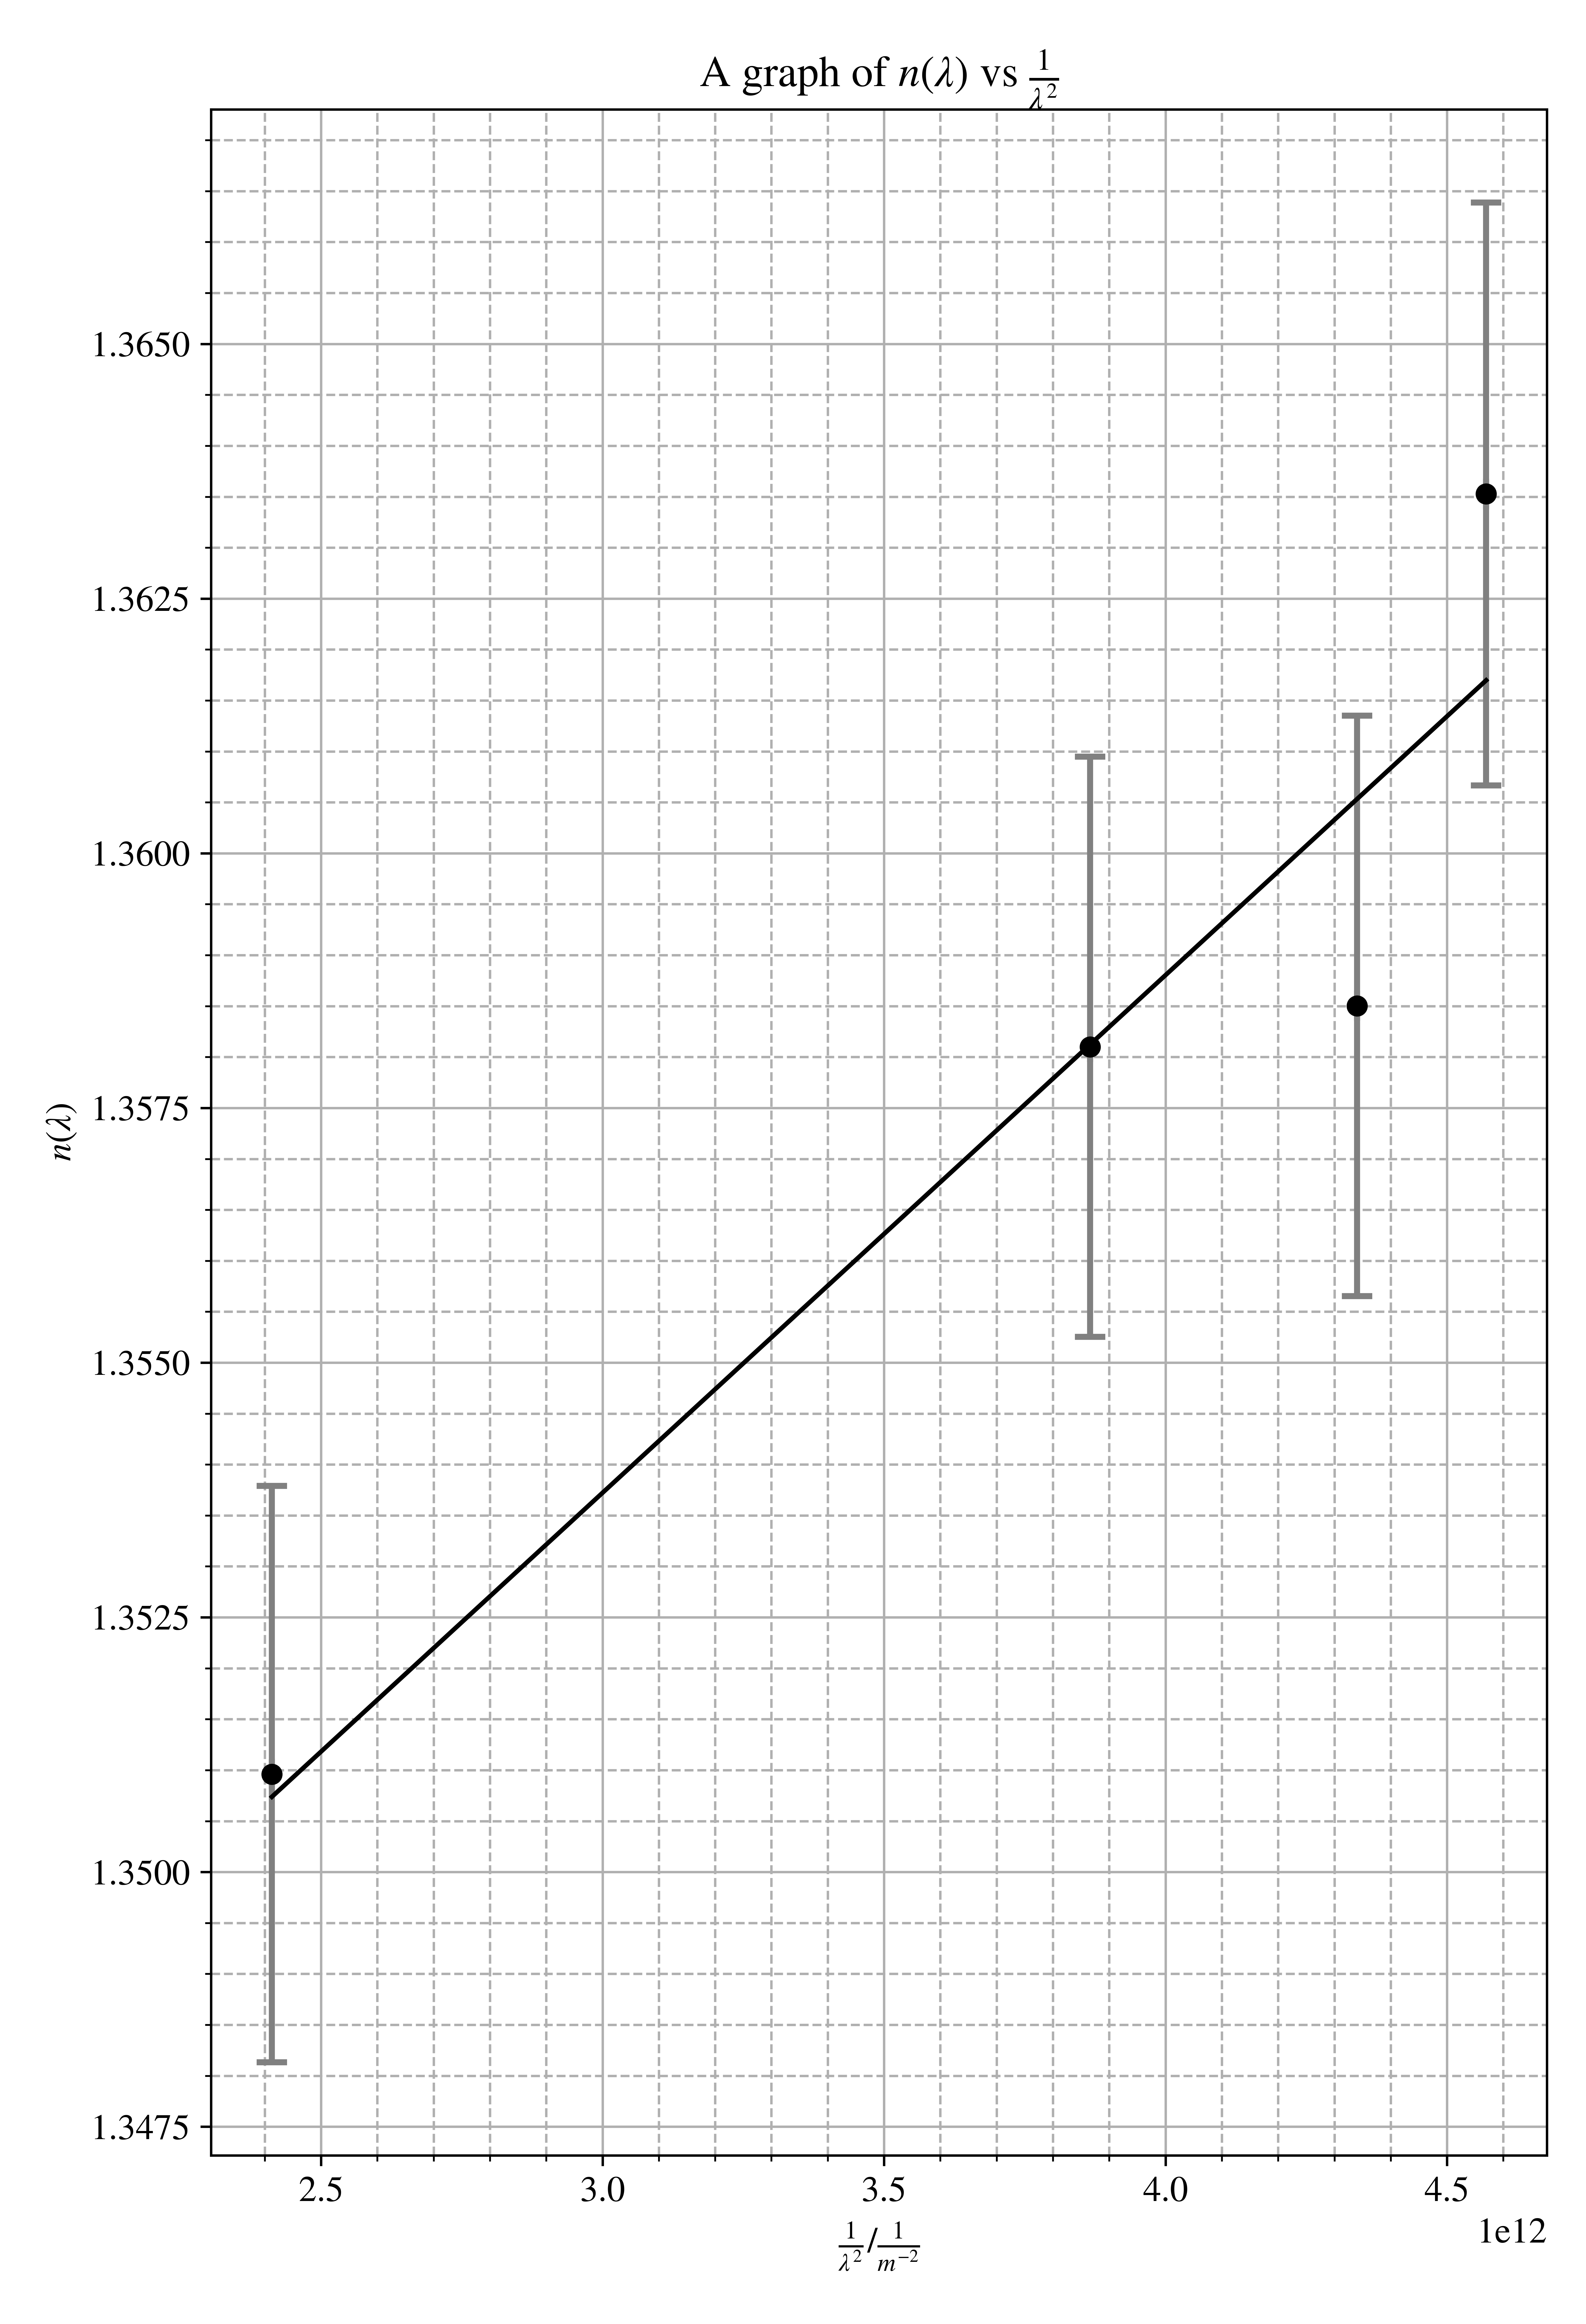
\includegraphics[width = \textwidth]{Plot1.png}
    \caption{$n(\lambda)$ vs $\frac{1}{\lambda^2}$}
    \label{fig:Plot}
\end{figure}

Graph is on page \pageref{fig:Plot}.

\section*{Calculations}
The data gathered in the experiment was read by the program with the following line of code:
\begin{minted}{python}
    data = pd.read_excel('Experiment 8.xlsx').
\end{minted}
The angles of the telescope used to determine the apex angle were read and converted by the program to radians with the following lines of code:
\begin{minted}{py}
    apexA = np.deg2rad(data['apexA'])
    apexAp = np.deg2rad(data['apexAp'])
    apexB = np.deg2rad(data['apexB'])
    apexBp = np.deg2rad(data['apexBp']),
\end{minted}
the equation to calculate the angle between the symmetric lines used were:
\begin{align*}
    \theta_1&=\frac{|A-A'|}{2}\,,\\
    \theta_2&=\frac{|B-B'|}{2}\,,
\end{align*}
where $A$ and $B$ are the angles read on the first unfrosted side of the prism and $A'$ and $B'$ were the second set of angles on the other unfrosted side of the prism. Thus the apex angle $\alpha$, was calculated using the following equation:
\begin{equation*}
    \alpha = \frac{\theta_1+\theta_2}{2}\,,
\end{equation*}
this was done through the following line of code:
\begin{minted}{py}
    alpha = ((np.absolute(apexA-apexAp)/2)+(np.absolute(apexB-apexBp)/2))/2 .
\end{minted}
In order to calculate the minimum deviation $\delta_m$ the following lines of code were used:
\begin{minted}{py}
    RedA = np.absolute(np.deg2rad(data['redA']-data['redAp']))/2
    RedB = np.absolute(np.deg2rad(data['redB']-data['redBp']))/2
    devRed = (RedA+RedB)/4

    GreenA = np.absolute(np.deg2rad(data['greenA']-data['greenAp']))/2
    GreenB = np.absolute(np.deg2rad(data['greenB']-data['greenBp']))/2
    devGreen = (GreenA+GreenB)/4

    CyanA = np.absolute(np.deg2rad(data['cyanA']-data['cyanAp']))/2
    CyanB = np.absolute(np.deg2rad(data['cyanB']-data['cyanBp']))/2
    devCyan = (CyanA+CyanB)/4

    BlueA = np.absolute(np.deg2rad(data['blueA']-data['blueAp']))/2
    BlueB = np.absolute(np.deg2rad(data['blueB']-data['blueBp']))/2
    devBlue = (BlueA+BlueB)/4 ,
\end{minted}
the final angle was halved again thus resulting in the division by 4, as the angle measured between the two line was between the zeroth order and the observed fringe. In order to calculate the refractive index of the material as a function of the wavelength of the fringe colour the following equation was used:
\begin{equation*}
    n(\lambda) = \frac{\sin{\left(\frac{\alpha + \delta_m}{2}\right)}}{\sin{\left(\frac{\alpha}{2}\right)}}\,.
\end{equation*}
This was done through the following lines of code:
\begin{minted}{py}
    nRed = np.sin((alpha + devRed)/2)/np.sin(alpha/2)
    nGreen = np.sin((alpha + devGreen)/2)/np.sin(alpha/2)
    nCyan = np.sin((alpha + devCyan)/2)/np.sin(alpha/2)
    nBlue = np.sin((alpha + devBlue)/2)/np.sin(alpha/2).
\end{minted}
The equation for Cauchy's Formula is as follows:
\begin{equation*}
    n(\lambda)=A+\frac{B}{\lambda^2}\,,
\end{equation*}
this was set to match the straight line equation $y = mx + c$, and on comparison $y = n(\lambda)$, $x = \frac{1}{\lambda^2}$, $m = B$ and $c = A$. Therefore in order to calculate the $\frac{1}{\lambda^2}$ the following lines of code were used:
\begin{minted}{py}
    xRed = 1/(6.438e-7)**2
    xGreen = 1/(5.086e-7)**2
    xCyan = 1/(4.80e-7)**2
    xBlue = 1/(4.678e-7)**2 .
\end{minted}
In order to plot the straight line graph the following lines of code were used:
\begin{minted}{py}
    coeffs, cov = np.polyfit(X, Y, deg=1, cov=True)
    polyfunct = np.poly1d(coeffs)
    trendline = polyfunct(X).
\end{minted}
By calling the correct position in the coeffs array it was found that A was found to be 1.34 and B was found to be \qty{5.08d-15}{\metre\squared}. In order to calculate the error for the reading so as to produce the errorbars, the following equations were used:

\begin{align*}
    \Delta \theta_1 &= \sqrt{\frac{\partial \theta_1}{\partial A}(\Delta A)^2+\frac{\partial \theta_1}{\partial A'}(\Delta A')^2}\,,\\
    \Delta \theta_2 &= \sqrt{\frac{\partial \theta_2}{\partial B}(\Delta B)^2+\frac{\partial \theta_2}{\partial B'}(\Delta B')^2}\,,\\
    \Delta \alpha &= \sqrt{\frac{\partial \alpha}{\partial \theta_1}(\Delta \theta_1)^2+\frac{\partial \alpha}{\partial \theta_2}(\Delta \theta_2)^2}\,,\\
    \Delta \delta_{colour} &= \sqrt{\frac{\partial \delta_{colour}}{\partial A}(\Delta A)^2+\frac{\partial \delta_{colour}}{\partial B}(\Delta B)^2}\,,\\
    \Delta n(\lambda) &= \sqrt{\frac{\partial n(\lambda)}{\partial \alpha}(\Delta \alpha)^2+\frac{\partial n(\lambda)}{\partial \delta_{colour}}(\Delta \delta_{colour})^2}\,.
\end{align*}

In order to calculate all of the errors the following lines of code were used:
\begin{minted}{py}
    def terror(c, d, dA):
        a = Symbol('a')
        b = Symbol('b')
        equation = ((a-b)/2)
        diffa = Derivative(equation, a)
        diffb = Derivative(equation, b)
        da = diffa.doit()
        db = diffb.doit()
        dc = da.subs({a: c, b: d}).evalf()
        dd = db.subs({a: c, b: d}).evalf()
        return sqrt((dc * dA) ** 2 + (dd * dA) ** 2)

    def aerror(e, f, dapexA, dapexB):
        a = Symbol('a')
        b = Symbol('b')
        equation = ((a+b)/2)
        diffa = Derivative(equation, a)
        diffb = Derivative(equation, b)
        da = diffa.doit()
        db = diffb.doit()
        de = da.subs({a: e, b: f}).evalf()
        df = db.subs({a: e, b: f}).evalf()
        return sqrt((de * dapexA) ** 2 + (df * dapexB) ** 2)

    def nerror(g, h, err, err2):
        a = Symbol('a')
        b = Symbol('b')
        equation = (sin((a+b)/2))/(sin(a/2))
        diffa = Derivative(equation, a)
        diffb = Derivative(equation,b)
        da = diffa.doit()
        db = diffb.doit()
        dg = da.subs({a : g, b : h}).evalf()
        dh = db.subs({a : g, b : h}).evalf()
        return sqrt((dg * err) ** 2 + (dh * err2) ** 2)

    def verror(i, h, err, err2):
        a = Symbol('a')
        b = Symbol('b')
        equation = (a+b)/4
        diffa = Derivative(equation, a)
        diffb = Derivative(equation, b)
        da = diffa.doit()
        db = diffb.doit()
        di = da.subs({a : i, b : h}).evalf()
        dh = db.subs({a : i, b : h}).evalf()
        return sqrt((di * err) ** 2 + (dh * err2) ** 2) 
    
    dapexA = terror(apexA, apexAp, dA)
    dapexB = terror(apexB, apexBp, dB)
    dalpha = aerror(dapexA, dapexB, dapexA, dapexB)

    vred = verror(RedA, RedB, dA, dB)
    vgreen = verror(GreenA, GreenB, dA, dB)
    vcyan = verror(CyanA, CyanB, dA, dB)
    vblue = verror(BlueA, BlueB, dA, dB)

    dnred = nerror(alpha,devRed,dalpha,vred)
    dngreen = nerror(alpha,devGreen,dalpha,vgreen)
    dncyan = nerror(alpha,devCyan,dalpha,vcyan)
    dnblue = nerror(alpha,devBlue,dalpha,vblue),
\end{minted}
the functions describe the partial derivation with respect to the individual changing components. Thus, the errorbars were plotted along with the graph. By calling the correct position in the covariance matrix the errors for both A and B were obtained. Thus, A was determined to be \num{1.34} \textpm \num{4.50d-3}, and B was found to be \num{5.08d-15} \textpm \qty{1.16d-15}{\metre\squared}. The actual values for both A and B were given during the experiment, which were defined as being equal to \num{1.5220} and \qty{4.59d-15}{\metre\squared} respectively. Thus, with these values the accuracy and precision of the results obtained could be calculated with the following equations:
\begin{align*}
    \text{Accuracy} &= \frac{\text{Experimental Value}}{\text{Actual Value}} \times 100\% \\
    \\
    \text{Precision}&=\frac{\text{Combined Error}}{\text{Experimental Value}} \times 100\% \,,
\end{align*}
these were calculated with the following lines of code:
\begin{minted}{py}
    accuracyA = (coeffs[1]/A)*100
    accuracyB = ((coeffs[0]/B)-1)*100
    precisionA = (aerr/coeffs[1])*100
    precisionB = (berr/coeffs[0])*100 ,
\end{minted}
which resulted that the value for A had an accuracy of 87.94\% and a precision of 0.34\%, while the result for B had an accuracy of 10.70\% and a precision of 22.75\%.

\section*{Discussion}
The constant A was found to be \num{1.34} \textpm \num{4.50d-3} while the actual value was quoted to be \num{1.5220}, while the constant B was found to be \num{5.08d-15} \textpm \qty{1.16d-15}{\metre\squared} when the actual value was \qty{4.59d-15}{\metre\squared}. This gave rise to constant A having a precision of $0.34\%$ and an accuracy of $87.94\%$ and constant B having a precision of $22.75\%$ and an accuracy of $10.70\%$. The low precision value for the constant A can be attributed to the precautions taken when doing the experiment also the fact that the spectrometer used had the small adjust feature which helped in positioning the crosshair as much as possible on the centre of the light ray observed from the lamp. However, it should be noted that the accuracy was either below the 90\% cut off point in the case of A, while for B it was above the 10\% cut off point. The main error for these values is the fact that the prism used had a chipped corner and thus, affecting all the readings and results obtained. Another value that should be noted is the high value of the precision for constant B which once again can be attributed to the fact that the prism used had a chipped corner. Additionally another error that should be taken into consideration was the fact that in order to see the values on the verniers of the spectrometer a lamp and a lens were used, therefore the values read off the verniers might not have been read at eye level, thus, introducing more errors to these readings. These errors can be noted in the graph in figure \ref{fig:Plot}, as the errorbars shown here are quite sizeable when compared to the scale taken on the y-axis. Also one should note that some of the values in the plot do not directly lie on the line of best fit, further indicating that some of the values used were not obtained precisely. 

\medskip
\noindent
Light spreading out when passing through a prism is called dispersion. Dispersion is when a narrow beam of white light is refracted by a prism, spreading out the light into bands of different colours. This occurs because the colour of the fringe with the shorter wavelength will be refracted more than the other fringes thus separating the colours from the white light \parencite{muncaster}. Diffraction on the other hand is when waves, such as light, pass through a slit which is parallel to the direction of travel. If the slit is of the same length to the wavelength of the waves, the waves will spread to regions that would be in shadow if the waves were travelling in straight lines. However, if the slit length is larger than the wavelength the effect is much less pronounced \parencite{muncaster}. 

\medskip
\noindent
The main similarities between the two phenomena are that both of them, when using white light, will depend on the angle of deviation and heavily depend on the wavelength of the light waves \parencite{hecht_2017}. The main differences between the two phenomena are that the velocity of the waves does not change in diffraction while in dispersion it decreases. Diffraction can be obtained when using monochromatic light while dispersion cannot. Diffraction does not depend on the refractive index of the material while dispersion heavily depends on the refractive index \parencite{hecht_2017}.

\section*{References}
\printbibliography[heading=none]

\section*{Appendix}
\begin{minted}{python}
import numpy as np
import pandas as pd
import matplotlib.pyplot as plt
from sympy import *
from math import sqrt

# inputting data from excel sheet
data = pd.read_excel('Experiment 8.xlsx')
# converting all angles into radians
apexA = np.deg2rad(data['apexA'])
apexAp = np.deg2rad(data['apexAp'])
apexB = np.deg2rad(data['apexB'])
apexBp = np.deg2rad(data['apexBp'])
# working out the apex angle
alpha = ((np.absolute(apexA-apexAp)/2)+(np.absolute(apexB-apexBp)/2))/2

# defining minimum readability and actual values
dA = 1/120
dB = 1/120
A = 1.5220
B = 4.59e-15

# finding the 1/wavelength**2 values
xRed = 1/(6.438e-7)**2
xGreen = 1/(5.086e-7)**2
xCyan = 1/(4.80e-7)**2
xBlue = 1/(4.678e-7)**2

# finding the minimum deviance angle of all colours
RedA = np.absolute(np.deg2rad(data['redA']-data['redAp']))/2
RedB = np.absolute(np.deg2rad(data['redB']-data['redBp']))/2
devRed = (RedA+RedB)/4

GreenA = np.absolute(np.deg2rad(data['greenA']-data['greenAp']))/2
GreenB = np.absolute(np.deg2rad(data['greenB']-data['greenBp']))/2
devGreen = (GreenA+GreenB)/4

CyanA = np.absolute(np.deg2rad(data['cyanA']-data['cyanAp']))/2
CyanB = np.absolute(np.deg2rad(data['cyanB']-data['cyanBp']))/2
devCyan = (CyanA+CyanB)/4

BlueA = np.absolute(np.deg2rad(data['blueA']-data['blueAp']))/2
BlueB = np.absolute(np.deg2rad(data['blueB']-data['blueBp']))/2
devBlue = (BlueA+BlueB)/4

nRed = np.sin((alpha + devRed)/2)/np.sin(alpha/2)
nGreen = np.sin((alpha + devGreen)/2)/np.sin(alpha/2)
nCyan = np.sin((alpha + devCyan)/2)/np.sin(alpha/2)
nBlue = np.sin((alpha + devBlue)/2)/np.sin(alpha/2)

# defining the y-axis and x-axis arrays
Y = np.hstack([nRed, nGreen, nCyan, nBlue])
X = np.array([xRed, xGreen, xCyan, xBlue])

# defining the partial derivative function for errors
def terror(c, d, dA):
    a = Symbol('a')
    b = Symbol('b')
    equation = ((a-b)/2)
    diffa = Derivative(equation, a)
    diffb = Derivative(equation, b)
    da = diffa.doit()
    db = diffb.doit()
    dc = da.subs({a: c, b: d}).evalf()
    dd = db.subs({a: c, b: d}).evalf()
    return sqrt((dc * dA) ** 2 + (dd * dA) ** 2)

def aerror(e, f, dapexA, dapexB):
    a = Symbol('a')
    b = Symbol('b')
    equation = ((a+b)/2)
    diffa = Derivative(equation, a)
    diffb = Derivative(equation, b)
    da = diffa.doit()
    db = diffb.doit()
    de = da.subs({a: e, b: f}).evalf()
    df = db.subs({a: e, b: f}).evalf()
    return sqrt((de * dapexA) ** 2 + (df * dapexB) ** 2)

def nerror(g, h, err, err2):
    a = Symbol('a')
    b = Symbol('b')
    equation = (sin((a+b)/2))/(sin(a/2))
    diffa = Derivative(equation, a)
    diffb = Derivative(equation,b)
    da = diffa.doit()
    db = diffb.doit()
    dg = da.subs({a : g, b : h}).evalf()
    dh = db.subs({a : g, b : h}).evalf()
    return sqrt((dg * err) ** 2 + (dh * err2) ** 2)

def verror(i, h, err, err2):
    a = Symbol('a')
    b = Symbol('b')
    equation = (a+b)/4
    diffa = Derivative(equation, a)
    diffb = Derivative(equation, b)
    da = diffa.doit()
    db = diffb.doit()
    di = da.subs({a : i, b : h}).evalf()
    dh = db.subs({a : i, b : h}).evalf()
    return sqrt((di * err) ** 2 + (dh * err2) ** 2)

# finding the errors for y-axis and x-axis values
dapexA = terror(apexA, apexAp, dA)
dapexB = terror(apexB, apexBp, dB)
dalpha = aerror(dapexA, dapexB, dapexA, dapexB)

vred = verror(RedA, RedB, dA, dB)
vgreen = verror(GreenA, GreenB, dA, dB)
vcyan = verror(CyanA, CyanB, dA, dB)
vblue = verror(BlueA, BlueB, dA, dB)

dnred = nerror(alpha,devRed,dalpha,vred)
dngreen = nerror(alpha,devGreen,dalpha,vgreen)
dncyan = nerror(alpha,devCyan,dalpha,vcyan)
dnblue = nerror(alpha,devBlue,dalpha,vblue)

# defining the error array for the y-axis
deltaY = np.hstack([dnred, dngreen, dncyan, dnblue])

# finding the line of best for the data gathered
coeffs, cov = np.polyfit(X, Y, deg=1, cov=True)
polyfunct = np.poly1d(coeffs)
trendline = polyfunct(X)

# finding the error for the coefficients
aerr = np.sqrt(cov[1][1])
berr = np.sqrt(cov[0][0])

# finding the accuracy for each coefficient
accuracyA = (coeffs[1]/A)*100
accuracyB = ((coeffs[0]/B)-1)*100
precisionA = (aerr/coeffs[1])*100
precisionB = (berr/coeffs[0])*100

# printing out the required information
print(f'A is found to be: {coeffs[1]:.2f} 
        with an error of: {aerr:.2e}')
print(f'A has an accuracy of: {accuracyA:.2f}% 
        and a precision of: {precisionA:.2f}%')
print(f'B is found to be: {coeffs[0]:.2e} 
        with an error of: {berr:.2e}')
print(f'B had an accuracy of: {accuracyB:.2f}% 
        and a precision of: {precisionB:.2f}%')

# defining the fonts and sizes to be used
plt.rcParams['font.family'] = 'STIXGeneral'
plt.rcParams['mathtext.fontset'] = 'stix'
plt.rcParams['font.size'] = 12
plt.rcParams['font.weight'] = 'normal'

# defining the figure size
plt.figure(figsize=(7.3, 10.7))

# plotting the figure
plt.errorbar(X, Y, xerr=0, yerr=deltaY, fmt='o', color='k', 
             elinewidth=2, capthick=2, capsize=5,
             ecolor='grey', label='Data Points')
plt.plot(X, trendline, color='k', label='Fit')
plt.minorticks_on()
plt.grid(visible=True, which='major', linestyle='-')
plt.grid(visible=True, which='minor', linestyle='--')
plt.title(r'A graph of $n(\lambda)$ vs $\frac{1}{\lambda^2}$')
plt.ylabel(r'$n(\lambda)$')
plt.xlabel(r'$\frac{1}{\lambda^2}$/$\frac{1}{m^{-2}}$')
# removing excess space from figure
plt.tight_layout()
plt.savefig('Plot1.png', dpi=800)
plt.legend()
plt.show()
\end{minted}

\end{document}
